%\documentclass[11pt,a4paper]{article}
\documentclass[preview]{standalone}
\usepackage[utf8]{inputenc}
\usepackage{graphicx}
\usepackage{subcaption}
\newcommand{\figures}{./figure}

\begin{document}

\begin{figure}
    \centering
    \begin{subfigure}[b]{0.45\textwidth}
        \caption{}
        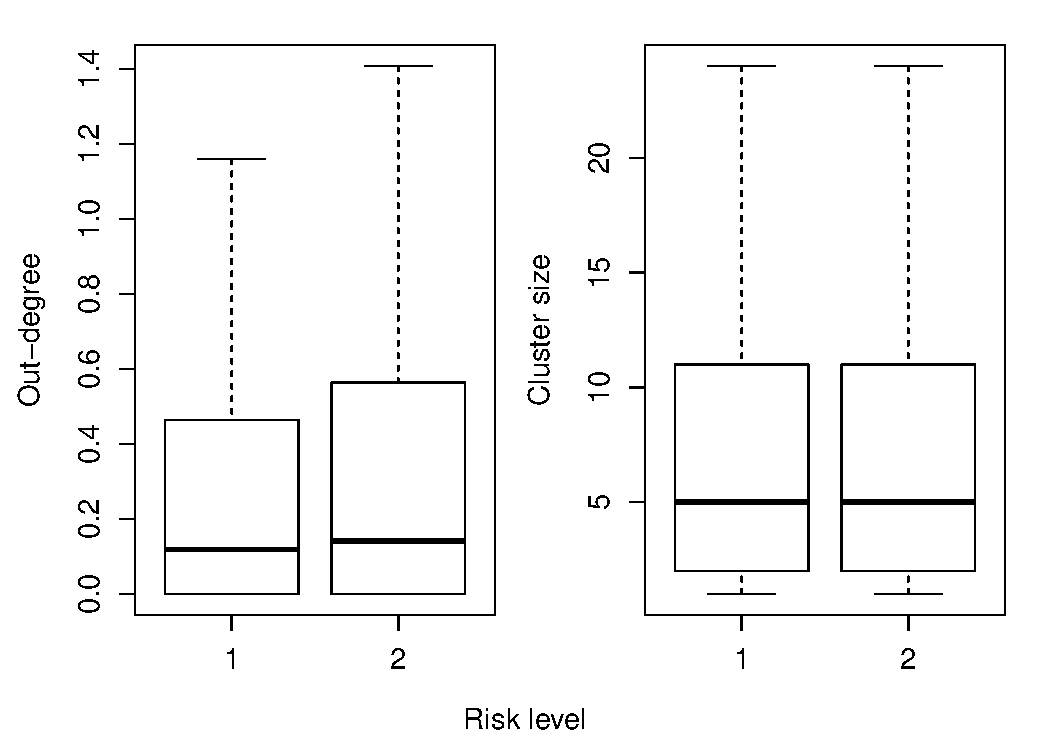
\includegraphics[width=\textwidth]{\figures/bp_base-1.pdf}
        \label{fig1a}
    \end{subfigure}
    ~ 
    \begin{subfigure}[b]{0.45\textwidth}
        \caption{}
        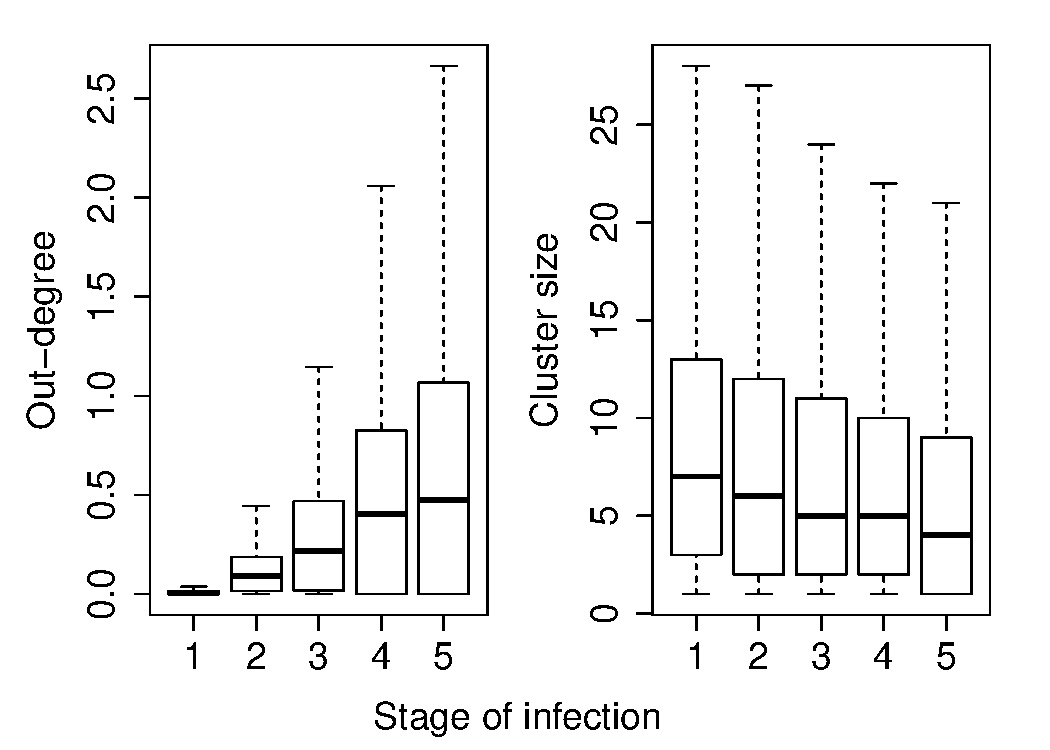
\includegraphics[width=\textwidth]{\figures/bp_base-3.pdf}        
        \label{fig1b}
    \end{subfigure}
    
    \begin{subfigure}[b]{0.45\textwidth}
        \caption{}
        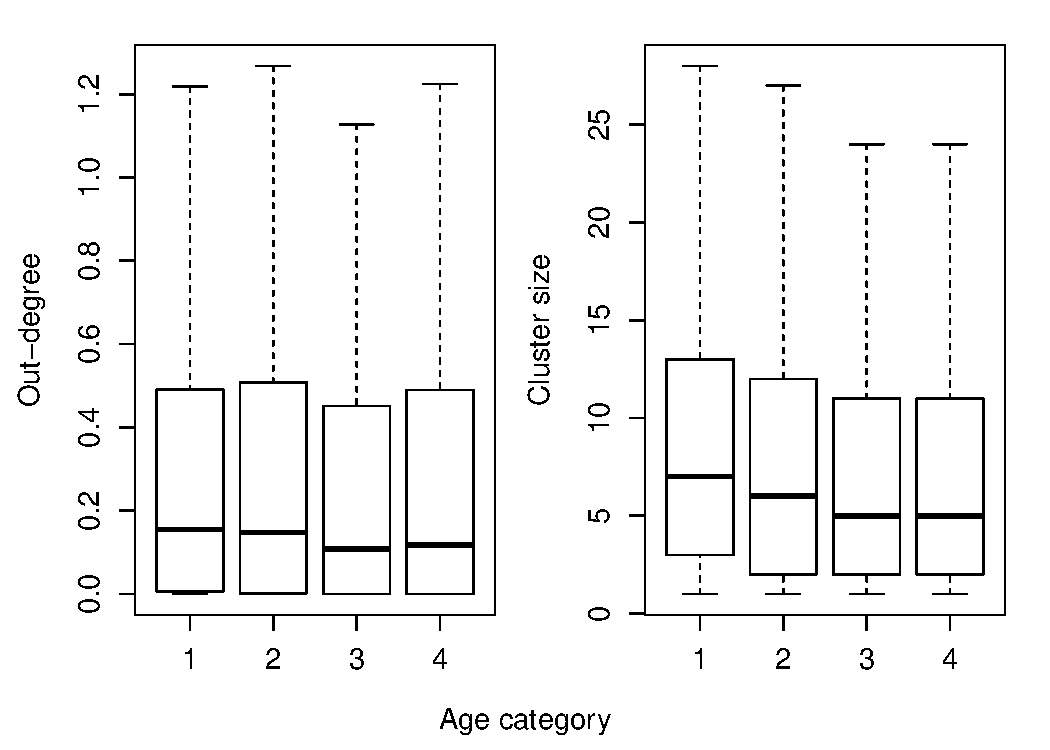
\includegraphics[width=\textwidth]{\figures/bp_base-2.pdf}        
        \label{fig1c}
    \end{subfigure}
   \caption[Distribution of out-degrees and cluster sizes by covariates]{Distribution of out-degrees and cluster sizes by (a) risk level: transmission rate was defined in the model as 10 times higher for risk level 2 relative to risk level 1; (b) stage of infection: relative transmission rates in the model were respectively 10, 1, 1, 1 and 3 for stages 1 to 5 of infection; (c) age category: transmission rates were equal for all 4 age categories in the model. Values are aggregated from 100 simulation replicates. Outliers are not shown. Distance threshold for clustering algorithm is 1.5\%.}
   \label{fig1}
\end{figure}

\end{document}